
\begin{figure}
\begin{center}
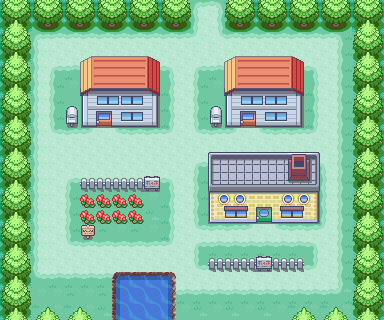
\includegraphics[width=2in]{PokemonPalletTown.png}
\end{center}
\caption{Pallet Town map from Pok\'{e}mon\cite{firered}} 
\end{figure}


We have created 6 symbols to be used to recreate maps for a popular video game
Pok\'{e}mon to ensure that our data set is sampled from some well defined distribution.

\begin{tabular}{llll}
Water & 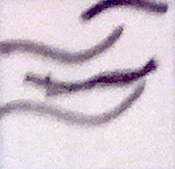
\includegraphics[width=.5in]{water.png} &
Grass & 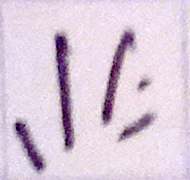
\includegraphics[width=.5in]{grass.png} \\
Rock & 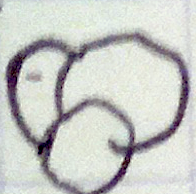
\includegraphics[width=.5in]{rocks.png} &
Tree & 
\includegraphics[width=.5in]{tree.png} \\
Dirt & 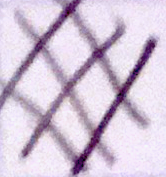
\includegraphics[width=.5in]{dirt.png} &
Sand & 
\includegraphics[width=.5in]{sand.png} \\
\end{tabular}


